\documentclass[polish,envcountsect,10pt]{beamer}
    \usepackage[T1]{fontenc}
    \usepackage{polski}
    \usepackage{babel}
    \usepackage{tikz}

    \usetheme{Warsaw}

    \title{Problem chińskiego listonosza (PCL)}
    \author{184657 Wojciech Panfil}
    \date{Gdańsk, 9.11.2023}
\begin{document}

\frame{\titlepage}

\begin{frame}{Krótkie przypomnienie o grafach}

Graf - matematyczna struktura danych składająca się z wierzchołków oraz krawędzi.
\medskip
\begin{itemize}
    \item Wierzchołki (węzły) reprezentowane są jako punkty i należą do zbioru $V$.
    \item Krawędzie (łuki) łączą wierzchołki i należą do zbioru $E$.
    \item Grafy mogą być skierowane (kierowane) lub nieskierowane (niekierowane).
\end{itemize}

\begin{center}

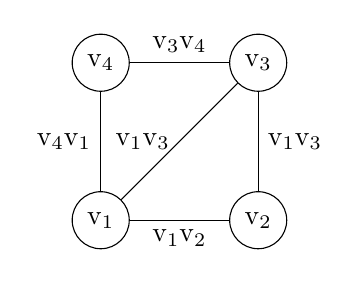
\begin{tikzpicture}
    % Wierzchołki
    \node[draw, circle] (v1) at (0,0) {v\textsubscript{1}};
    \node[draw, circle] (v2) at (2,0) {v$_2$};
    \node[draw, circle] (v3) at (2,2) {v$_3$};
    \node[draw, circle] (v4) at (0,2) {v$_4$};
    
  % Krawędzie z etykietami
  \draw (v1) -- (v2) node[midway, below] {v$_1$v$_2$};
  \draw (v2) -- (v3) node[midway, right] {v$_1$v$_3$};
  \draw (v3) -- (v4) node[midway, above] {v$_3$v$_4$};
  \draw (v4) -- (v1) node[midway, left] {v$_4$v$_1$};
  \draw (v1) -- (v3) node[midway, left] {v$_1$v$_3$};
\end{tikzpicture}

\end{center}

\begin{itemize}
    \item G = ($V$ , $E$)
    \item $V$ = \{v$_1$, v$_2$, v$_3$, v$_4$\}
    \item $E$ = \{v$_1$v$_2$, v$_1$v$_3$, v$_3$v$_4$, v$_4$v$_1$, v$_1$v$_3$\}
\end{itemize}

\end{frame}


\end{document}